\documentclass[tikz,border=6pt]{standalone}
\usepackage[T1]{fontenc}
\usepackage{lmodern}
\usepackage{xcolor}
\usetikzlibrary{arrows.meta,fit,calc,positioning}

\definecolor{cliBg}{RGB}{232,242,252}
\definecolor{cliBrd}{RGB}{45,105,175}
\definecolor{srvBg}{RGB}{254,240,225}
\definecolor{srvBrd}{RGB}{195,95,25}
\definecolor{shmBg}{RGB}{230,245,225}
\definecolor{shmBrd}{RGB}{55,130,45}
\definecolor{ipcBg}{RGB}{255,246,215}
\definecolor{ipcBrd}{RGB}{185,35,35}
\definecolor{ioBg}{RGB}{242,242,245}
\definecolor{ioBrd}{RGB}{90,90,100}

\tikzset{
  box/.style={
    draw=#1, line width=0.8pt, rounded corners=3pt,
    align=center, font=\sffamily\footnotesize,
    inner sep=5pt, minimum height=1.15cm
  },
  cblock/.style={box=cliBrd, fill=cliBg},
  sblock/.style={box=srvBrd, fill=srvBg},
  shmblock/.style={box=shmBrd, fill=shmBg},
  ipcblock/.style={box=ipcBrd, fill=ipcBg},
  ioblock/.style={box=ioBrd, fill=ioBg},
  groupbox/.style={
    draw=#1, line width=1.1pt, dashed, rounded corners=5pt,
    inner sep=9pt
  },
  grouplabel/.style={
    font=\sffamily\bfseries\small, inner sep=3pt
  },
  arr/.style={-{Latex[length=2.4mm,width=1.8mm]}, line width=0.9pt, black!75},
  ipcarr/.style={-{Latex[length=2.5mm,width=1.9mm]}, line width=1.15pt, ipcBrd},
  ipcboth/.style={{Latex[length=2.4mm,width=1.8mm]}-{Latex[length=2.4mm,width=1.8mm]}, line width=1.15pt, ipcBrd},
  shmarr/.style={-{Latex[length=2.4mm,width=1.8mm]}, line width=1.0pt, dashed, shmBrd},
  lbl/.style={font=\sffamily\scriptsize, inner sep=1.5pt}
}

\begin{document}
\hyphenpenalty=10000\relax\exhyphenpenalty=10000\relax
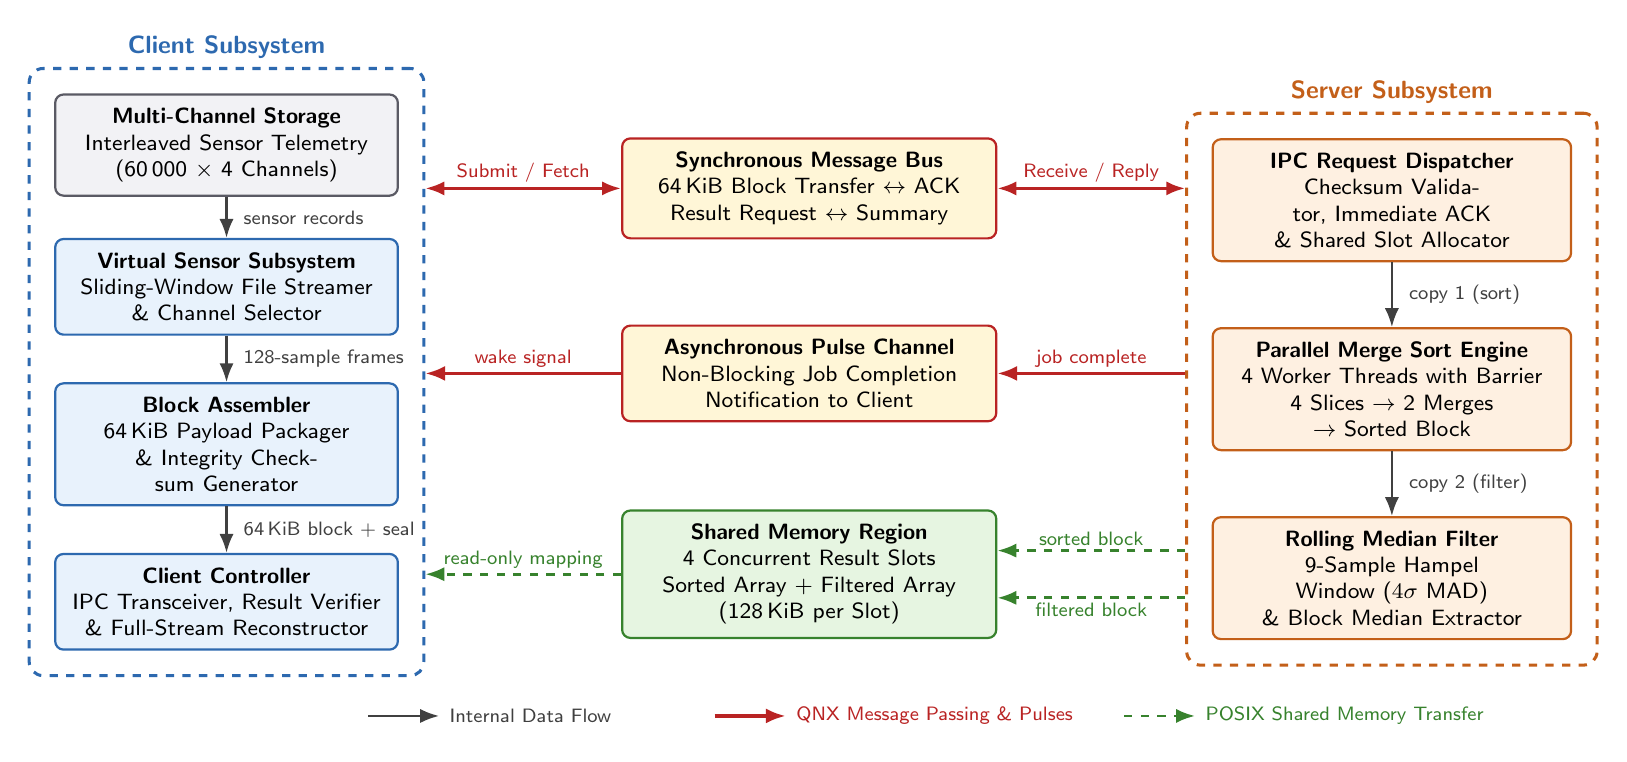
\begin{tikzpicture}

% ==================== LEFT: CLIENT SUBSYSTEM ====================
\node[ioblock, text width=4.0cm] (disk) at (0, 2.55) {
  \textbf{Multi-Channel Storage}\\
  Interleaved Sensor Telemetry\\
  (60\,000 $\times$ 4 Channels)
};

\node[cblock, text width=4.0cm] (sensor) at (0, 0.75) {
  \textbf{Virtual Sensor Subsystem}\\
  Sliding-Window File Streamer\\
  \& Channel Selector
};

\node[cblock, text width=4.0cm] (loader) at (0, -1.25) {
  \textbf{Block Assembler}\\
  64\,KiB Payload Packager\\
  \& Integrity Checksum Generator
};

\node[cblock, text width=4.0cm] (cipc) at (0, -3.25) {
  \textbf{Client Controller}\\
  IPC Transceiver, Result Verifier\\
  \& Full-Stream Reconstructor
};

\node[groupbox=cliBrd, fit=(disk)(sensor)(loader)(cipc),
      label={[grouplabel, text=cliBrd]above:Client Subsystem}] (cligroup) {};

% ==================== CENTER: QNX IPC & SHARED MEMORY ====================
\node[ipcblock, text width=4.4cm] (qnxmsg) at (7.4, 2.0) {
  \textbf{Synchronous Message Bus}\\
  64\,KiB Block Transfer $\leftrightarrow$ ACK\\
  Result Request $\leftrightarrow$ Summary
};

\node[ipcblock, text width=4.4cm] (qnxpulse) at (7.4, -0.35) {
  \textbf{Asynchronous Pulse Channel}\\
  Non-Blocking Job Completion\\
  Notification to Client
};

\node[shmblock, text width=4.4cm] (shm) at (7.4, -2.9) {
  \textbf{Shared Memory Region}\\
  4 Concurrent Result Slots\\
  Sorted Array + Filtered Array\\
  (128\,KiB per Slot)
};

% ==================== RIGHT: SERVER SUBSYSTEM ====================
\node[sblock, text width=4.2cm] (sipc) at (14.8, 1.85) {
  \textbf{IPC Request Dispatcher}\\
  Checksum Validator, Immediate ACK\\
  \& Shared Slot Allocator
};

\node[sblock, text width=4.2cm] (sort) at (14.8, -0.55) {
  \textbf{Parallel Merge Sort Engine}\\
  4 Worker Threads with Barrier\\
  4 Slices $\rightarrow$ 2 Merges $\rightarrow$ Sorted Block
};

\node[sblock, text width=4.2cm] (median) at (14.8, -2.95) {
  \textbf{Rolling Median Filter}\\
  9-Sample Hampel Window ($4\sigma$ MAD)\\
  \& Block Median Extractor
};

\node[groupbox=srvBrd, fit=(sipc)(sort)(median),
      label={[grouplabel, text=srvBrd]above:Server Subsystem}] (srvgroup) {};

% ==================== CONNECTIONS ====================
% Client internal
\draw[arr] (disk.south) -- node[lbl, right, xshift=1.5mm]{sensor records} (sensor.north);
\draw[arr] (sensor.south) -- node[lbl, right, xshift=1.5mm]{128-sample frames} (loader.north);
\draw[arr] (loader.south) -- node[lbl, right, xshift=1.5mm]{64\,KiB block + seal} (cipc.north);

% Server internal
\draw[arr] (sipc.south) -- node[lbl, right, xshift=1.5mm]{copy 1 (sort)} (sort.north);
\draw[arr] (sort.south) -- node[lbl, right, xshift=1.5mm]{copy 2 (filter)} (median.north);

% Cross-process IPC & Shared Memory
\draw[ipcboth] (cligroup.east |- qnxmsg.west) -- node[lbl, above]{Submit / Fetch} (qnxmsg.west);
\draw[ipcboth] (qnxmsg.east) -- node[lbl, above]{Receive / Reply} (srvgroup.west |- qnxmsg.east);

\draw[ipcarr] (srvgroup.west |- qnxpulse.east) -- node[lbl, above]{job complete} (qnxpulse.east);
\draw[ipcarr] (qnxpulse.west) -- node[lbl, above]{wake signal} (cligroup.east |- qnxpulse.west);

\draw[shmarr] ([yshift=0.3cm]srvgroup.west |- shm.east) -- node[lbl, above]{sorted block} ([yshift=0.3cm]shm.east);
\draw[shmarr] ([yshift=-0.3cm]srvgroup.west |- shm.east) -- node[lbl, below]{filtered block} ([yshift=-0.3cm]shm.east);
\draw[shmarr] (shm.west) -- node[lbl, above]{read-only mapping} (cligroup.east |- shm.west);

% Legend bar at bottom
\begin{scope}[shift={(1.8,-4.7)}]
  \draw[arr] (0,0) -- (0.9,0) node[right, font=\sffamily\scriptsize]{Internal Data Flow};
  \draw[ipcarr] (4.4,0) -- (5.3,0) node[right, font=\sffamily\scriptsize]{QNX Message Passing \& Pulses};
  \draw[shmarr] (9.6,0) -- (10.5,0) node[right, font=\sffamily\scriptsize]{POSIX Shared Memory Transfer};
\end{scope}

\end{tikzpicture}
\end{document}